\chapter{Spot}
Spot was first presented in 2004 \cite{2}. It was purely a library until Spot 1.0 \cite{1}, when
command-line tools for LTL manipulation and translation of LTL to some generalizations of Büchi Automata
have started to be distributed. Today, Spot 2.0 supports more tools with arbitrary acceptance conditions
as described in the Hanoi Omega Automata format (HOA) \cite{3} and python bindings usable in interactive
environments such as IPython/Jupyter \cite{4}.

\section{Structure}
The Spot project can be broken down into several parts, as shown in Figure~\ref{fig:arch}. Orange boxes are C/C++ libraries.
Red boxes are command-line program. Blue boxes are Python-related.
\begin{figure}[H]
 \centering
 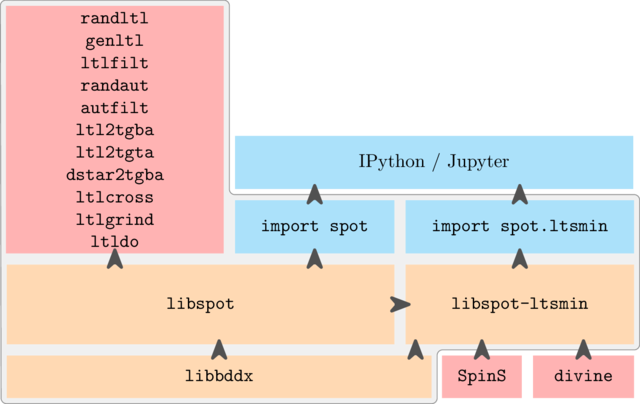
\includegraphics[scale=0.6]{img/arch.png}
 \caption{Architecture of Spot}
 \label{fig:arch}
\end{figure}
Spot is actually split in three libraries:
\begin{itemize}
 \item libbddx is a customized version of BuDDy for representing Binary Decision Diagrams which we use to
label transitions in automata, and to implement a few algorithms.
 \item libspot is the main library containing all data structures and algorithms.
 \item libspot-ltsmin contains code to interface with state-spaces generated as shared libraries by LTSmin.
\end{itemize}


\section{Command-line tools}
Spot 2.0 installs the following eleven command-line tools, that are designed to be combined as traditional
Unix tools.\\
\begin{figure}[H]
 \begin{tabular}{l c | m{8cm}}
  \multirow{13}{*}{SPOT 1.0}&randltl&Generates random LTL/PSL formulas\\
   &genltl&Generates LTL formulas from scalable patterns\\
   &ltlfilt&Filter, converts, and transforms LTL/PSL formulas\\
   &ltl2tgba&Translates LTL/PSL formulas into generalized Büchi automata\cite{7}, or deterministic parity
	     automata (new in 2.0)\\
   &ltl2tgta&Translates LTL/PSL formulas into Testing automata\cite{6}\\
   &ltlcross&Cross-compares LTL/PSL-to-automata translators to find bugs (works with arbitrary acceptance
	     conditions since Spot 2.0)\\
   \hline
   &ltlgrind&mutates LTL/PSL formulas to help reproduce bugs on smaller ones\\
   &dstar2tgba&converts ltl2dstar automata into Generalized Büchi automata\cite{14}\\
   &randaut&generates random $\omega$-automata\\
   &autfilt&filters, converts and transforms $\omega$-automata\\
   &ltldo&runs LTL/PSL formulas through other translators, providing uniform input and output interfaces\\
 \end{tabular}
 \caption{Spot tools description}
\end{figure}
As you see, the first six tools were introduced in Spot 1.0 \cite{1}, and have since received several updates. The other tools
were introduced after.

\section{The Python Interface}
Similar tasks can be performed in a more ''algorithm-friendly'' environment using the Python interface.
Combined with the IPython/Jupyter notebook \cite{4} (a web application for interactive programming), this
provides a nice environment for experiments, where automata and formulas are automatically displayed.

\section{Workflow}
Working on any project of the LRDE implies to follow some rules. That allows a better integration of each
member. Once a patch is ready, any member of the model checking team can re-read the patch and make
suggestions.

\subsection{Coding conventions}
As Spot is a free software, uniformity of the code matters a lot. Some coding conventions are used so that
the code looks homogeneous. Here are some points:
\begin{itemize}
 \item UTF-8 is used for non-ASCII characters.
 \item tabs are not used for indentation in c++ files, only spaces, in order to prevent issues with people
 assuming different tab widths.
 \item \#include with angle-brackets refers to public Spot headers (i.e those that will be installed, or
 system headers that are already installed).
 \item \# include with double quotes refer to private headers that are distributed with Spot.
 \item ... (see \url{https://gitlab.lrde.epita.fr/spot/spot/blob/master/HACKING} for more details)
\end{itemize}

\subsection{Git Versionning Tool}
The versionning tool used in Spot is Git. All development branches except 'master' and 'next' follows a particular naming convention:
\{initials\}/\{subject of work\}). This allows a quick glance to identify who works on which branch and on
what.

Concerning commits, large commits introducing a feature are preferred to many small commits covering
the same feature. Suppose that a new feature must be implemented and needs 3 key steps. Even if each step
is done in many commits during the development, at the end, it's better to squash commits so as to have
only 3 large commits representing the 3 key steps.

Also, if at any moment in turns out that a previous work
could have been done otherwise, any update must be applied directly to the commit concerned - each commit
must actually insert code in its final form.

\subsection{Adding Tests}
Any implementation done must be tested. For the purpose on one hand to avoid regression and on the other
hand to ensure the code runs as expected. All tests are located in the 'tests' folders. Must of them
are written in Python (using the python bindings) or shell script.

